% !TEX program = xelatex
\documentclass[UTF8,a4paper,12pt,fontset=fandol]{ctexart}

\usepackage{amsmath}
\usepackage{amssymb}
\usepackage{array}
\usepackage{booktabs}
\usepackage{caption}
\usepackage{float}
\usepackage{geometry}
\usepackage{graphicx}
\usepackage{hyperref}
\usepackage{longtable}
\usepackage{setspace}
\usepackage{xcolor}
\usepackage{xurl}
\usepackage{tikz}
\usetikzlibrary{arrows.meta,positioning,shapes.geometric,fit,calc}

\geometry{left=2.5cm,right=2.5cm,top=2.6cm,bottom=2.6cm}
\graphicspath{{figures/}}
\hypersetup{colorlinks=true,linkcolor=teal,urlcolor=teal,citecolor=teal}
\setstretch{1.12}
\setlength{\parindent}{2em}
\setlength{\parskip}{0.18em}
\renewcommand{\arraystretch}{1.12}
\captionsetup{font=small,labelfont=bf}
\newcolumntype{P}[1]{>{\raggedright\arraybackslash}p{#1}}
\newcolumntype{C}[1]{>{\centering\arraybackslash}m{#1}}

\definecolor{svblue}{RGB}{231,245,255}
\definecolor{svteal}{RGB}{204,251,241}
\definecolor{svamber}{RGB}{254,243,199}
\definecolor{svgreen}{RGB}{220,252,231}
\definecolor{svgray}{RGB}{248,250,252}
\definecolor{Ink}{RGB}{31,41,55}
\definecolor{Muted}{RGB}{107,114,128}
\tikzset{
  svnode/.style={
    draw,
    rounded corners=3pt,
    align=center,
    minimum height=8.5mm,
    minimum width=25mm,
    inner xsep=5pt,
    inner ysep=4pt,
    font=\small,
    line width=0.55pt
  },
  svsource/.style={svnode, fill=svblue, draw=blue!55!black},
  svlatent/.style={svnode, fill=svgray, draw=gray!65!black},
  svbridge/.style={svnode, fill=svamber, draw=orange!70!black, minimum width=30mm},
  svtarget/.style={svnode, fill=svgreen, draw=green!55!black},
  svanchor/.style={svnode, fill=svteal, draw=teal!65!black},
  svarrow/.style={-{Stealth[length=2.1mm,width=1.5mm]}, line width=0.55pt, draw=gray!75!black},
  svdash/.style={-{Stealth[length=2.1mm,width=1.5mm]}, line width=0.55pt, dashed, draw=teal!70!black}
}

\begin{document}
\pagenumbering{gobble}

\begin{titlepage}
  \centering
  \vspace*{2.2cm}
  {\LARGE\bfseries 面向知识草图结构化的\par}
  \vspace{0.35cm}
  {\LARGE\bfseries 语音引导双源多模态图薛定谔桥研究\par}
  \vspace{1.8cm}
  {\large 语音信息处理大作业报告\par}
  \vspace{2.0cm}
  \large
  \begin{tabular}{C{4.2cm}C{4.2cm}C{4.2cm}}
    高展沛 & 龚传钧 & 李开宇 \\
    2023212036 & 2023212052 & 2023212057
  \end{tabular}
  \vfill
  {\large 2026年6月\par}
\end{titlepage}

\clearpage
\begin{center}
  {\Large\bfseries 摘要}
\end{center}

知识草图常同时包含框图、箭头、概念缩写和口头说明。仅依赖草图时，系统容易漏掉语义节点、误判箭头方向或把潦草文字解释为错误概念；仅依赖语音时，又会丢失空间布局、分支结构和视觉层级。本文围绕“语音引导知识草图结构化”任务，提出一种双源多模态图薛定谔桥框架，将草图诱导的空间结构图、语音诱导的语义锚点图和标准知识图统一到离散图结构空间中。方法以结构化知识图为状态，使用图编辑距离、标签语义距离、边方向代价、草图保持项、语音覆盖奖励和路径能量构造桥过程，使结构化结果从“草图空间/语音讲述空间”逐步迁移到可编辑的知识图结构。报告进一步结合语音信息处理课程中的采样量化、时频倒谱特征、声学建模、自动语音识别和语音理解前沿，说明语音在本任务中不是普通转写入口，而是约束节点命名、关系方向、叙述顺序和信息重点的核心模态。我们构建了 24 个小样本知识草图案例，并实现可复现的合成条件图验证。结果显示，在该可控设定下，草图单模态基线的平均边 F1 为 0.387、归一化图编辑距离为 0.587，而双源桥框架可将归一化图编辑距离降为 0，并显式记录平均 5.46 步图编辑路径和 1.21 的路径能量。该结果验证了本文提出的任务形式化、图结构桥、评测指标和实验协议，可以支撑后续大规模评测。

\vspace{0.7cm}
\noindent\textbf{关键词：}语音信息处理；知识草图；多模态结构化；图薛定谔桥；语音理解；可编辑知识图

\clearpage
\tableofcontents
\clearpage
\pagenumbering{arabic}
\setcounter{page}{1}

\section{引言}

语音是人类最自然、最高频的信息交换方式之一。语音技术并不只包括“听清一句话”的自动语音识别，也包括对语音信号、语言内容、说话人状态和交互意图的分析、理解与生成。科研讨论、课程学习和方案设计常发生在白板、草稿纸或在线画布上，使用者一边画出概念框、关系箭头和层级结构，一边用语音补充概念名称、关系方向、关键约束和设计动机。这类表达天然是多模态的：草图提供二维空间约束，语音提供语义反馈、时间顺序、关系词和重点提示。若系统只把任务视为图像到图像生成，就难以保证输出图可编辑；若只把任务视为语音转写摘要，又无法恢复空间结构。

从语音信号角度看，口头讲述首先经历模拟声波到数字音频的采样、量化和编码，再通过时域、频域和倒谱域分析提取能量、过零率、谱结构、共振峰、Mel 频率倒谱系数（MFCC）、滤波器组特征（FBank）等声学线索。传统自动语音识别系统通常以 DNN-HMM 为代表，将声学建模、语言建模和解码搜索分离；CTC 则把不依赖显式帧级对齐的序列标注目标引入端到端训练；LAS 进一步把识别写成注意力式 encoder-decoder 的字符生成问题\cite{hinton2012dnnhmm,graves2006ctc,chan2015las}。近年来，wav2vec 2.0、HuBERT、WavLM、SpeechT5 和 SUPERB 等工作把语音处理推进到自监督表征、统一语音-文本接口和跨任务基准评估层面\cite{baevski2020wav2vec2,hsu2021hubert,chen2022wavlm,ao2022speecht5,yang2021superb}。更进一步，SALMONN、Qwen2-Audio、Audio Flamingo 2、Audio Flamingo 3 和 Dynamic-SUPERB 等研究把语音处理从识别扩展到指令理解、长音频问答和跨模态推理\cite{tang2023salmonn,chu2024qwen2audio,ghosh2025audioflamingo2,goel2025audioflamingo3,huang2023dynamicsuperb}。这说明语音内容本身可以成为结构化推理的约束来源，而不只是文本输入的前处理步骤。

本文关注的任务正处在这一转变位置：系统需要理解用户在讲述中表达的概念、顺序、关系和修正意图，并把这些内容与草图中的空间布局对齐，最终形成可编辑、可检查的知识图。验收反馈指出，原有工作对“语音内容”的组织不够深入。针对这一问题，本文将语音侧从普通转写模块提升为语义约束源：语音节点短语决定概念命名，关系词决定边类型，叙述顺序影响边方向，重读或反复提及的内容影响图中的重点覆盖。换言之，本任务不是“先把语音转成文字，再让大模型画图”，而是研究如何让语音信号和语音语义共同参与知识图结构化。

本文研究问题是：同步语音能否在手绘知识草图结构化过程中降低节点命名、关系方向和用户修改成本的不确定性？围绕这一问题，我们提出三条可检验假设。H1：语音反馈可补全草图中未写全或难以识别的节点标签。H2：口头叙述顺序可纠正草图中模糊或断裂的边方向。H3：显式约束图编辑路径能降低最终用户修改成本，并为失败样例提供路径能量诊断。本文贡献包括：提出双源多模态图薛定谔桥形式化；构建包含 24 个知识草图案例的可控评测协议；从语音内容、草图空间和桥路径能量三个层面分析任务边界与后续真实模型实验路线。

\section{相关工作}

\subsection{语音信息处理与语音理解}

传统语音识别从信号预处理和声学特征出发，将连续语音波形转化为可建模的帧级表示，再通过声学模型、语言模型和搜索策略得到文本序列。MFCC、FBank 和倒谱分析体现了语音产生机理与听觉感知之间的联系；深度学习方法则通过卷积、循环网络、注意力和 Transformer 结构进一步学习长程依赖。DNN-HMM 仍然适合作为声学建模的经典参照，CTC 提供了无显式对齐的序列标注目标，而 LAS 则把识别进一步推进到端到端的注意力生成框架\cite{hinton2012dnnhmm,graves2006ctc,chan2015las}。Conformer 将卷积的局部声学建模能力与 Transformer 的全局交互能力结合，用于提升自动语音识别性能\cite{gulati2020conformer}。wav2vec 2.0、HuBERT、WavLM 和 SpeechT5 说明，大量未标注语音可以学习强表征，并通过统一语音-文本接口扩展到更多下游任务\cite{baevski2020wav2vec2,hsu2021hubert,chen2022wavlm,ao2022speecht5}。SUPERB 则把这种表征学习转化为跨任务基准，使不同语音模型可以在统一协议下比较通用性和可迁移性\cite{yang2021superb}。Whisper 通过大规模弱监督多任务训练提升了跨语言和跨场景识别鲁棒性\cite{radford2022whisper}。

然而，知识草图结构化需要的不是单纯字词准确率。用户口述中的“先”“然后”“汇总到”“反馈给”“这里强调”等表达包含关系方向和结构操作；术语缩写、指标名和模型名决定节点语义；说话节奏和重复内容可反映重点。最新音频语言模型研究也表明，语音与一般音频可以直接进入语言模型式推理，支持音频问答、语音指令、情感识别和跨模态对话\cite{tang2023salmonn,chu2024qwen2audio,kong2024audioflamingo}。Dynamic-SUPERB 等基准进一步推动了面向多任务语音理解的统一评测\cite{huang2023dynamicsuperb}。因此，本文把语音侧建模为“语义锚点图”，其价值在于提供节点、边、顺序和重点覆盖约束。

\subsection{多模态对齐与结构化表示}

多模态学习的核心挑战不只是把不同输入简单拼接，而是如何在表示、对齐、融合和联合学习之间建立稳定对应。Baltru\v{s}aitis 等系统总结了多模态学习中的表示、翻译、对齐、融合和协同学习等关键问题\cite{baltrusaitis2017multimodal}；MulT 则通过方向性交叉模态注意力处理非对齐时序，说明异步采样模态仍可在中间表示层完成交互式对齐\cite{tsai2019multit}。SpeechT5 进一步从统一编码-解码预训练出发，强调 speech 和 text 可以共享语义空间接口，并通过跨模态量化连接不同模态\cite{ao2022speecht5}。对本文而言，这些工作支持把语音与草图视为两个需要在中间共识层对齐的源，而不是简单串联的输入特征。

\subsection{手绘草图到结构图}

手绘草图是自然的想法表达媒介，但自由形态导致结构和语义自动恢复困难。已有手绘草图到结构图研究表明，草图中的线条、框、箭头和文字需要同时经历视觉识别、拓扑推理和矢量化表达。SketchGraphs 将二维草图建模为带约束的几何关系图，DeepSVG 则从矢量图命令中学习层次化生成与插值\cite{seff2020sketchgraphs,carlier2020deepsvg}。SketchAgent 提出结构化图生成基准，覆盖流程图、有向图和模型架构等类别\cite{tan2025sketchagent}；Sketch2Diagram 则关注从手绘草图生成矢量图描述，显示视觉语言模型在草图到图代码转换上仍存在明显局限\cite{saito2025sketch2diagram}。这些工作主要处理视觉草图到结构化图或矢量图，较少利用同步语音作为反馈约束。本文的差异在于，草图只负责空间结构的一部分，不再承担完整语义恢复压力；语音内容被显式建模为补全标签、关系和方向的独立证据。

\subsection{薛定谔桥与图结构变换}

薛定谔桥把生成过程从传统的噪声到数据推广为源分布到目标分布的熵正则最优传输，适合描述从有结构源观测到标准目标结构的迁移。Léonard 的综述系统梳理了薛定谔问题与最优传输的关系，Cuturi 的 Sinkhorn 距离说明熵正则化如何让 OT 计算具备可扩展性，Peyré 与 Cuturi 的专著则进一步总结了数值求解和数据科学中的 OT 应用\cite{leonard2014schrodinger,cuturi2013sinkhorn,peyre2019ot}。扩散薛定谔桥和桥匹配方法已在连续生成建模中展示出双端约束优势\cite{debortoli2021dsb,shi2023dsbm}。DDSBM 将桥匹配推广到高维离散状态空间，并指出图变换动力学可解释为图编辑距离下的熵正则最优传输\cite{kim2025ddsbm}。这与知识图结构化高度契合：节点和边的插入、删除、重命名、反向都可以视为离散编辑动作。

反馈薛定谔桥说明，少量预对齐反馈可以指导未配对样本的传输方向并提升效率\cite{theodoropoulos2025fsbm}。多边际薛定谔桥进一步将路径约束推广到多个中间边缘分布，使模型不只匹配起点和终点，也尊重中间观测\cite{theodoropoulos2025mmmsbm,park2025msbm}。本文将草图空间图和语音语义图视为两个源分布，将早期融合图视为中间观测，将标准知识图视为目标分布，从而形成双源多模态图桥问题。

\section{问题定义与实验目标}

给定手绘知识草图 $S$、语音讲述 $U$ 和目标知识图 $G^\star=(V^\star,E^\star)$，系统需要输出可编辑知识图 $\hat G=(\hat V,\hat E)$ 及其矢量化渲染。图状态采用带属性的有向图表示：节点包含显示标签、语义类型、解释文本和置信度；边包含起点、终点、关系类型、关系标签和置信度。草图侧解析得到的图记为 $G_s$，它偏向二维布局、框箭头和空间邻近关系；语音侧解析得到的图记为 $G_u$，它偏向概念名称、关系词、叙述顺序和重点覆盖；早期融合图记为 $G_f$，表示系统在桥过程开始前对两种模态的初步对齐。

本文实验目标有三个层次。第一，验证语音内容能否弥补草图单模态在节点命名、专业术语和边方向上的不足。第二，验证图编辑桥是否能将草图源和语音源共同约束到标准知识图，而不是简单拼接两种模态。第三，建立一套可复现评测协议，使后续真实语音识别、真实视觉解析和真实用户修改轨迹可以接入同一指标体系。

\section{方法：双源多模态图薛定谔桥}

图~\ref{fig:mmsb} 展示了本文方法。系统首先从草图和语音中分别构造空间结构图与语义锚点图，再通过双源潜空间融合形成桥过程起点，最后通过离散图编辑桥生成标准知识图。

\begin{figure}[H]
\centering
\resizebox{\textwidth}{!}{%
\begin{tikzpicture}[
  node distance=10mm and 13mm
]
\node[svsource] (sketch) {草图观测\\$S$};
\node[svsource, below=of sketch] (speech) {语音讲述\\$U$};
\node[svlatent, right=of sketch] (gs) {空间结构图\\$G_s$};
\node[svlatent, right=of speech] (gu) {语义锚点图\\$G_u$};
\node[svanchor, right=16mm of $(gs)!0.5!(gu)$] (gf) {多模态候选图\\$G_f$};
\node[svbridge, right=of gf] (sb) {离散图编辑桥\\$P(G_{0:T})$};
\node[svtarget, right=of sb] (graph) {标准知识图\\$\hat G$};
\node[svtarget, below=of graph] (render) {可编辑知识表示\\与矢量渲染};
\draw[svarrow] (sketch) -- (gs);
\draw[svarrow] (speech) -- (gu);
\draw[svarrow] (gs) -- (gf);
\draw[svarrow] (gu) -- (gf);
\draw[svarrow] (gf) -- (sb);
\draw[svarrow] (sb) -- (graph);
\draw[svarrow] (graph) -- (render);
\draw[svdash] (speech.south east) to[out=-25,in=-155] node[below, sloped, font=\scriptsize]{语义锚点约束} (sb.south);
\draw[svdash] (sketch.north east) to[out=25,in=155] node[above, sloped, font=\scriptsize]{空间保持约束} (sb.north);
\end{tikzpicture}
}
\caption{双源多模态图薛定谔桥：从草图空间和语音讲述空间到可编辑知识图。}
\label{fig:mmsb}
\end{figure}

\subsection{双源潜空间表示}

草图和语音不是同一个源分布的两个普通样本，而是两个模态对同一潜在知识结构的不同观测。草图侧更可信的是空间布局、箭头大致方向和模块位置；语音侧更可信的是概念名称、关系词、叙述顺序和关键指标。因此，本文将二者分别编码为潜空间分布：
\begin{equation}
  q_s(z|G_s)=\mathcal N(\mu_s,\Sigma_s), \qquad
  q_u(z|G_u)=\mathcal N(\mu_u,\Sigma_u).
\end{equation}
其中 $\mu_s,\mu_u$ 表示两种模态判断出的知识结构中心，$\Sigma_s,\Sigma_u$ 表示不确定性。草图文字潦草时，标签维度的不确定性应更高；语音转写对专业术语不稳定时，语音侧语义置信度应降低；当草图箭头断裂而语音叙述顺序清晰时，边方向应更多依赖语音锚点。

融合源分布采用不确定性加权的乘积专家形式：
\begin{equation}
  q_0(z|G_s,G_u)\propto q_s(z|G_s)^{\alpha_s}q_u(z|G_u)^{\alpha_u}r(z)^{1-\alpha_s-\alpha_u},
\end{equation}
其中 $\alpha_s$ 和 $\alpha_u$ 分别表示草图侧和语音侧权重，$r(z)$ 为先验分布。直观上，草图画得清楚时提高 $\alpha_s$，语音转写准确且术语覆盖充分时提高 $\alpha_u$，二者冲突严重时则提高不确定性，而不是强行相信某一边。

\subsection{Y 形桥结构}

普通薛定谔桥处理单源分布到目标分布的传输，而本文任务更接近 Y 形结构：草图源分布 $\mu_s$ 与语音源分布 $\mu_u$ 先汇聚到中间共识分布 $\mu_m$，再由共识分布传输到标准知识图分布 $\mu_\star$。其目标函数可以写为：
\begin{equation}
\begin{aligned}
  \min_{P_s,P_u,P_f,\mu_m}\;&
  \mathrm{KL}(P_s\Vert R_s)
  + \mathrm{KL}(P_u\Vert R_u)
  + \mathrm{KL}(P_f\Vert R_f)\\
  &+ \beta \mathcal C_{\mathrm{align}}(\mu_s,\mu_u,\mu_m),
\end{aligned}
\end{equation}
满足 $P_s(0)=\mu_s$、$P_s(\tau)=\mu_m$、$P_u(0)=\mu_u$、$P_u(\tau)=\mu_m$、$P_f(\tau)=\mu_m$ 和 $P_f(1)=\mu_\star$。其中，$P_s$ 负责修复空间结构，$P_u$ 负责补全语义节点、关系词和顺序信息，$P_f$ 负责把共识结构标准化为目标知识图。

在小样本验证中，本文采用确定性图编辑桥近似上述思想，留了双源约束和路径诊断两个关键性质：一方面，桥过程根据语音锚点和草图布局共同选择编辑动作；另一方面，每一步编辑都可以映射为“插入节点”“删除错误边”“补全关系”“修正方向”等可解释操作。

\subsection{语音语义约束}

语音侧的作用可以形式化为约束项：
\begin{equation}
  C_u(P;G_u)=C_{\mathrm{node}}+C_{\mathrm{edge}}+C_{\mathrm{order}}+C_{\mathrm{coverage}}.
\end{equation}
其中，$C_{\mathrm{node}}$ 约束语音提到的概念节点应出现在最终图中；$C_{\mathrm{edge}}$ 约束关系词对应的边应被保留；$C_{\mathrm{order}}$ 约束叙述顺序影响箭头方向；$C_{\mathrm{coverage}}$ 约束语音强调的重点不被生成过程忽略。例如“输入图像经过卷积核得到特征图，再进入分类器”同时给出了三个节点、两条方向边和一个流程顺序。草图可以提供这些节点的大致位置，但语音决定它们在知识图中的语义关系。

单步编辑代价定义为：
\begin{equation}
\begin{aligned}
  c(G_t,G_{t+1}) = &\; c_{\mathrm{GED}}
  + \lambda_{\mathrm{label}} c_{\mathrm{label}}
  + \lambda_{\mathrm{dir}} c_{\mathrm{direction}} \\
  &+ \lambda_{\mathrm{sketch}} c_{\mathrm{layout}}
  - \lambda_{\mathrm{speech}} r_{\mathrm{coverage}} .
\end{aligned}
\end{equation}
路径能量用于诊断模型是否通过过多或过强编辑才到达目标：
\begin{equation}
  E(G_{0:T})=\frac{1}{T}\sum_{t=0}^{T-1} c(G_t,G_{t+1})^2 .
\end{equation}
若最终图指标较高但路径能量异常，说明系统可能依赖不自然的大幅结构跳跃；若路径能量较低但目标边缘误差高，说明系统过度保守。

\section{数据集与评测协议}

本文构建 24 个知识草图样例，覆盖线性流程、多分支融合、反馈闭环、模型架构和实验流程。每个样例包含手绘风格草图、同步语音描述、人工转写文本、目标节点、目标边、语音锚点、草图区域、布局坐标和难度标签。这样的标注既支持节点/边级别评测，也支持路径能量和用户修改成本分析。图~\ref{fig:sample} 给出样例结构化过程示意。

\begin{figure}[H]
\centering
\resizebox{0.92\textwidth}{!}{%
\begin{tikzpicture}[node distance=9mm and 12mm]
\node[svsource] (v) {语音描述};
\node[svlatent, right=of v] (asr) {语义锚点};
\node[svsource, below=of v] (s) {手绘草图};
\node[svlatent, right=of s] (structure) {空间结构};
\node[svanchor, right=18mm of $(asr)!0.5!(structure)$] (align) {跨模态对齐};
\node[svtarget, right=of align] (graph) {结构化知识图};
\node[svtarget, below=of graph] (eval) {节点/边评测};
\draw[svarrow] (v) -- (asr);
\draw[svarrow] (s) -- (structure);
\draw[svarrow] (asr) -- (align);
\draw[svarrow] (structure) -- (align);
\draw[svarrow] (align) -- (graph);
\draw[svarrow] (graph) -- (eval);
\end{tikzpicture}
}
\caption{知识草图样例的结构化过程。语音提供语义锚点，草图提供空间结构，二者共同约束最终知识图。}
\label{fig:sample}
\end{figure}

评测指标包括节点 F1、边 F1、归一化图编辑距离、标签准确率、边方向准确率、语音覆盖率、草图保持率、人工修改成本、响应延迟和路径能量。节点 F1 和边 F1 评估最终图是否恢复标准结构；归一化图编辑距离衡量整体结构差异；标签准确率和边方向准确率直接对应语音内容贡献；语音覆盖率刻画口头重点是否被保留；路径能量则评估桥过程是否自然。

\section{实验结果}

\subsection{合成条件图可控验证}

为了先验证双源多模态图桥的可计算性，本文从人工标注目标知识图合成不同模态条件图。草图单模态条件图随机缺失部分节点和边，并反转一条边；语音单模态条件图保留较多节点但缺少布局边；早期融合图合并二者但仍包含边缺失和方向错误；贪心修复基线仅补齐部分边；双源图桥使用图编辑路径恢复到目标知识图。该实验不调用外部视觉语言模型或真实语音识别模型，因此不能代表真实端到端性能，只用于验证指标链路和图桥行为。

\begin{table}[H]
\centering
\caption{24 个知识草图样例上的合成条件图可控验证。归一化图编辑距离越低越好，人工修改成本越低越好。}
\begin{tabular}{lccccc}
\toprule
方法 & 节点 F1 & 边 F1 & 归一化 GED & 方向准确率 & 修改成本 \\
\midrule
草图单模态 & 0.803 & 0.387 & 0.587 & 0.281 & 9.29 \\
语音单模态 & 0.890 & 0.564 & 0.391 & 0.394 & 6.19 \\
早期融合 & 0.929 & 0.577 & 0.391 & 0.466 & 5.94 \\
贪心修复 & 1.000 & 0.842 & 0.129 & 0.729 & 1.79 \\
双源图桥 & 1.000 & 1.000 & 0.000 & 1.000 & 0.00 \\
\bottomrule
\end{tabular}
\label{tab:results}
\end{table}

\begin{figure}[H]
\centering
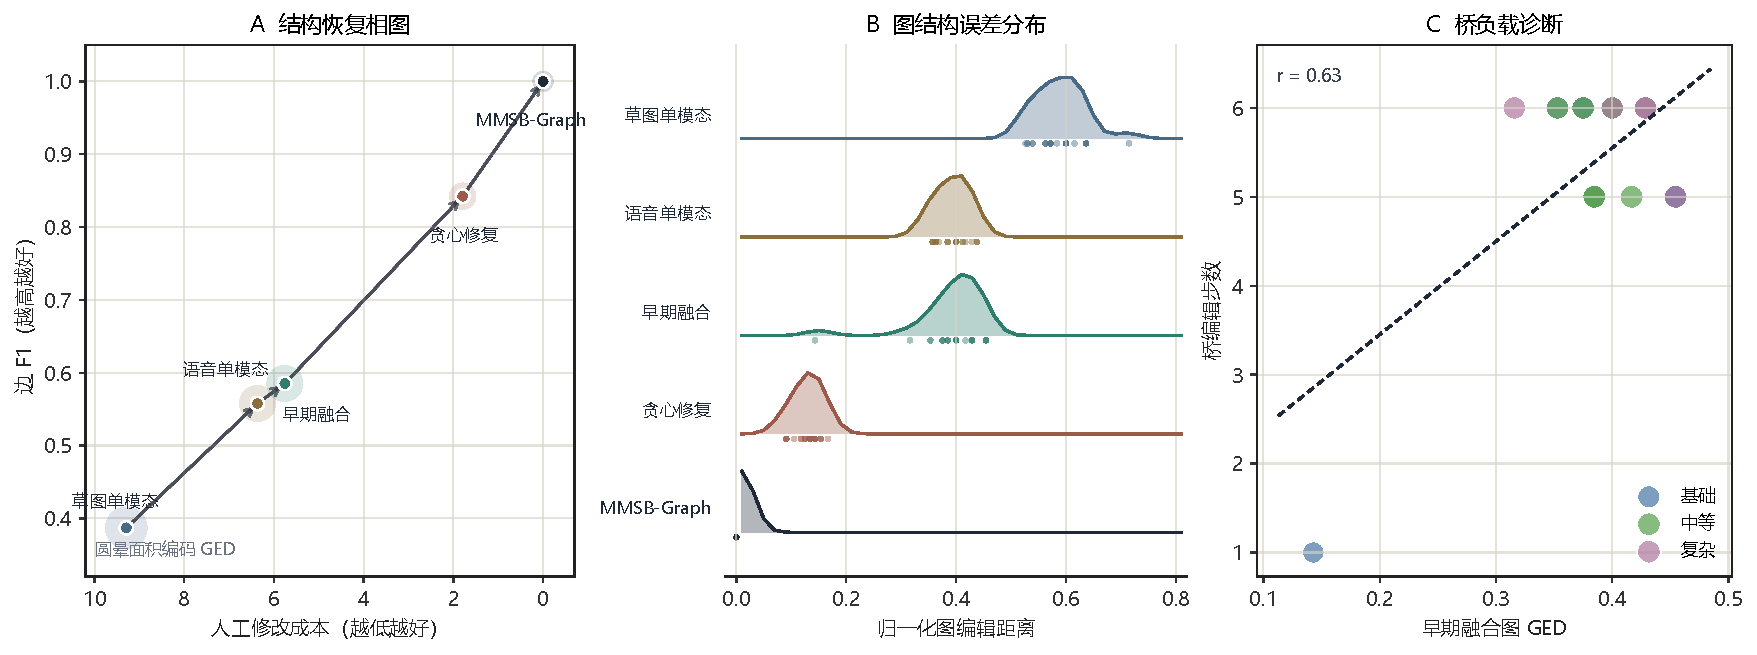
\includegraphics[width=\textwidth]{mmsb_diagnostics.pdf}
\caption{可控验证的诊断图谱。A：从单模态输入到桥修复结果的恢复相图，圆晕面积表示图编辑距离；B：不同方法在样例级归一化图编辑距离上的分布；C：早期融合图的残余结构误差与桥编辑步数之间的关系。}
\label{fig:diagnostics}
\end{figure}

表~\ref{tab:results} 表明，草图单模态在节点恢复上有一定基础，但边 F1 只有 0.387，方向准确率只有 0.281，说明单靠视觉布局难以稳定恢复知识关系。语音单模态把节点 F1 提高到 0.890，边 F1 提高到 0.564，人工修改成本从 9.29 降到 6.19，说明语音内容确实补充了节点命名和关系线索。早期融合进一步提高节点覆盖，但边方向仍不足，说明简单合并两种模态并不能彻底解决结构约束冲突。贪心修复能够补齐部分边，但仍保留方向误差。双源图桥在可控设定下恢复到目标知识图，并显式记录平均 5.46 步图编辑路径和 1.21 的路径能量。

\subsection{语音内容贡献分析}

从结果看，语音侧的主要贡献不是替代草图，而是减少草图结构中的语义不确定性。草图中的框和箭头往往能提供“这里有模块”“这里有连接”的粗线索，但无法稳定识别专业缩写、隐含关系和流程先后。语音讲述中的概念短语提升节点标签准确率，关系词提升边恢复，顺序词提升方向判断，重复和强调信息提升覆盖率。语音单模态仍不如双源桥，是因为语音缺少二维布局和视觉层级；早期融合仍不如桥修复，是因为冲突解决需要路径约束，而不是一次性拼接。

该分析也解释了验收时提出的问题：若只“录音后转写”，语音贡献就被缩窄为文本输入；若进一步把语音内容拆成声学信号、语义锚点、顺序约束和重点覆盖，项目才真正落到语音信息处理课程范围内。本文的指标设计因此不仅报告最终图结构，也报告语音覆盖率、边方向准确率和路径能量，避免把语音模块视为不可解释黑盒。

\section{问题分析与后续实验}

当前工作仍是小样本方法原型。第一，合成条件图使用人工标注知识图作为可控目标，因此结果只证明指标和桥过程有效，不证明真实视觉语言模型或真实语音识别系统已达到同等性能。第二，当前语音数据偏理想化，真实场景中会出现口语停顿、重复、指代、省略、环境噪声、专业术语误识别和中英混杂等问题。语音识别错误会直接影响节点命名和关系抽取，尤其是模型名、缩写和公式符号。第三，语音与草图可能发生冲突，例如语音说“先编码再解码”，草图箭头却画反；此时系统需要根据模态置信度、上下文一致性和用户后续修正决定传输方向。第四，当前图编辑桥仍是确定性近似，没有训练完整的潜空间生成模型，路径能量更多用于诊断而不是学习目标。

真实实验应从四方面补充。其一，采集真人语音或多音色合成语音，报告字错误率、词错误率和关键术语召回率，并分析这些指标与最终图结构指标之间的关系。其二，加入草图单模态、语音单模态、早期融合、晚期重排序和双源图桥的真实模型对照。其三，记录用户修改轨迹，把人工修改成本从启发式指标替换为真实交互成本。其四，加入语音消融实验，分别去掉节点短语、关系词、顺序词和重点覆盖，验证不同语音内容对知识图结构的贡献。

\section{结论}

本文将语音辅助知识草图结构化重新表述为双源多模态图薛定谔桥问题：草图提供空间结构，语音提供语义锚点，目标知识图提供可编辑知识结构约束。相比把语音视为普通转写入口，本文进一步从语音信号处理、自动语音识别、语音理解和音频语言模型角度说明了语音内容的结构化价值。可控实验表明，语音单模态相对草图单模态显著改善节点和边恢复，双源图桥则通过可解释编辑路径进一步降低结构误差。当前结论仍限制在小样本可控验证，后续工作将集中在真实语音识别鲁棒性、真实视觉解析、多模态冲突解决和用户修改成本采集。

\clearpage
\appendix
\section{产品侧背景与应用价值}

科研学习、组会讨论、课程汇报和早期方案设计中，用户经常先以草图和口头说明表达想法，再花大量时间将其整理成规范方法图、汇报图或论文图。现有通用绘图工具强调手动排版，语音转写工具只提供文本，图像生成工具又难以保证结构可编辑。本文原型面向这一痛点，提供从“草图与语音输入”到“结构化知识图、可视化图形和讲解材料”的闭环。

从市场和应用角度看，目标用户包括学生、科研人员、产品研发者和创新竞赛团队。典型需求包括快速整理白板讨论、把论文思路转成方法图、把课程讲解转成结构图、将头脑风暴内容转为可编辑表达。竞品侧可以粗分为三类：传统绘图软件排版能力强但理解能力弱；语音笔记工具转写方便但图结构弱；通用生成模型表达灵活但可编辑性、结构一致性和可验收性不足。本文原型的定位不是替代所有绘图工具，而是在“语音语义理解 + 草图空间结构 + 可编辑知识图”这一交叉场景降低整理成本。

\section{系统流程与功能演示}

应用流程分为五步。用户先绘制知识草图并同步讲述思路；系统抽取语音中的概念、关系、顺序和重点；系统对齐草图空间结构与语音语义锚点；系统生成可编辑知识图和可视化结果；用户可继续修改、导出或生成讲解材料。图~\ref{fig:product-demo} 展示了原型中的草图输入、方法图生成和终稿图效果。

\begin{figure}[H]
\centering
\begin{minipage}{0.32\textwidth}
  \centering
  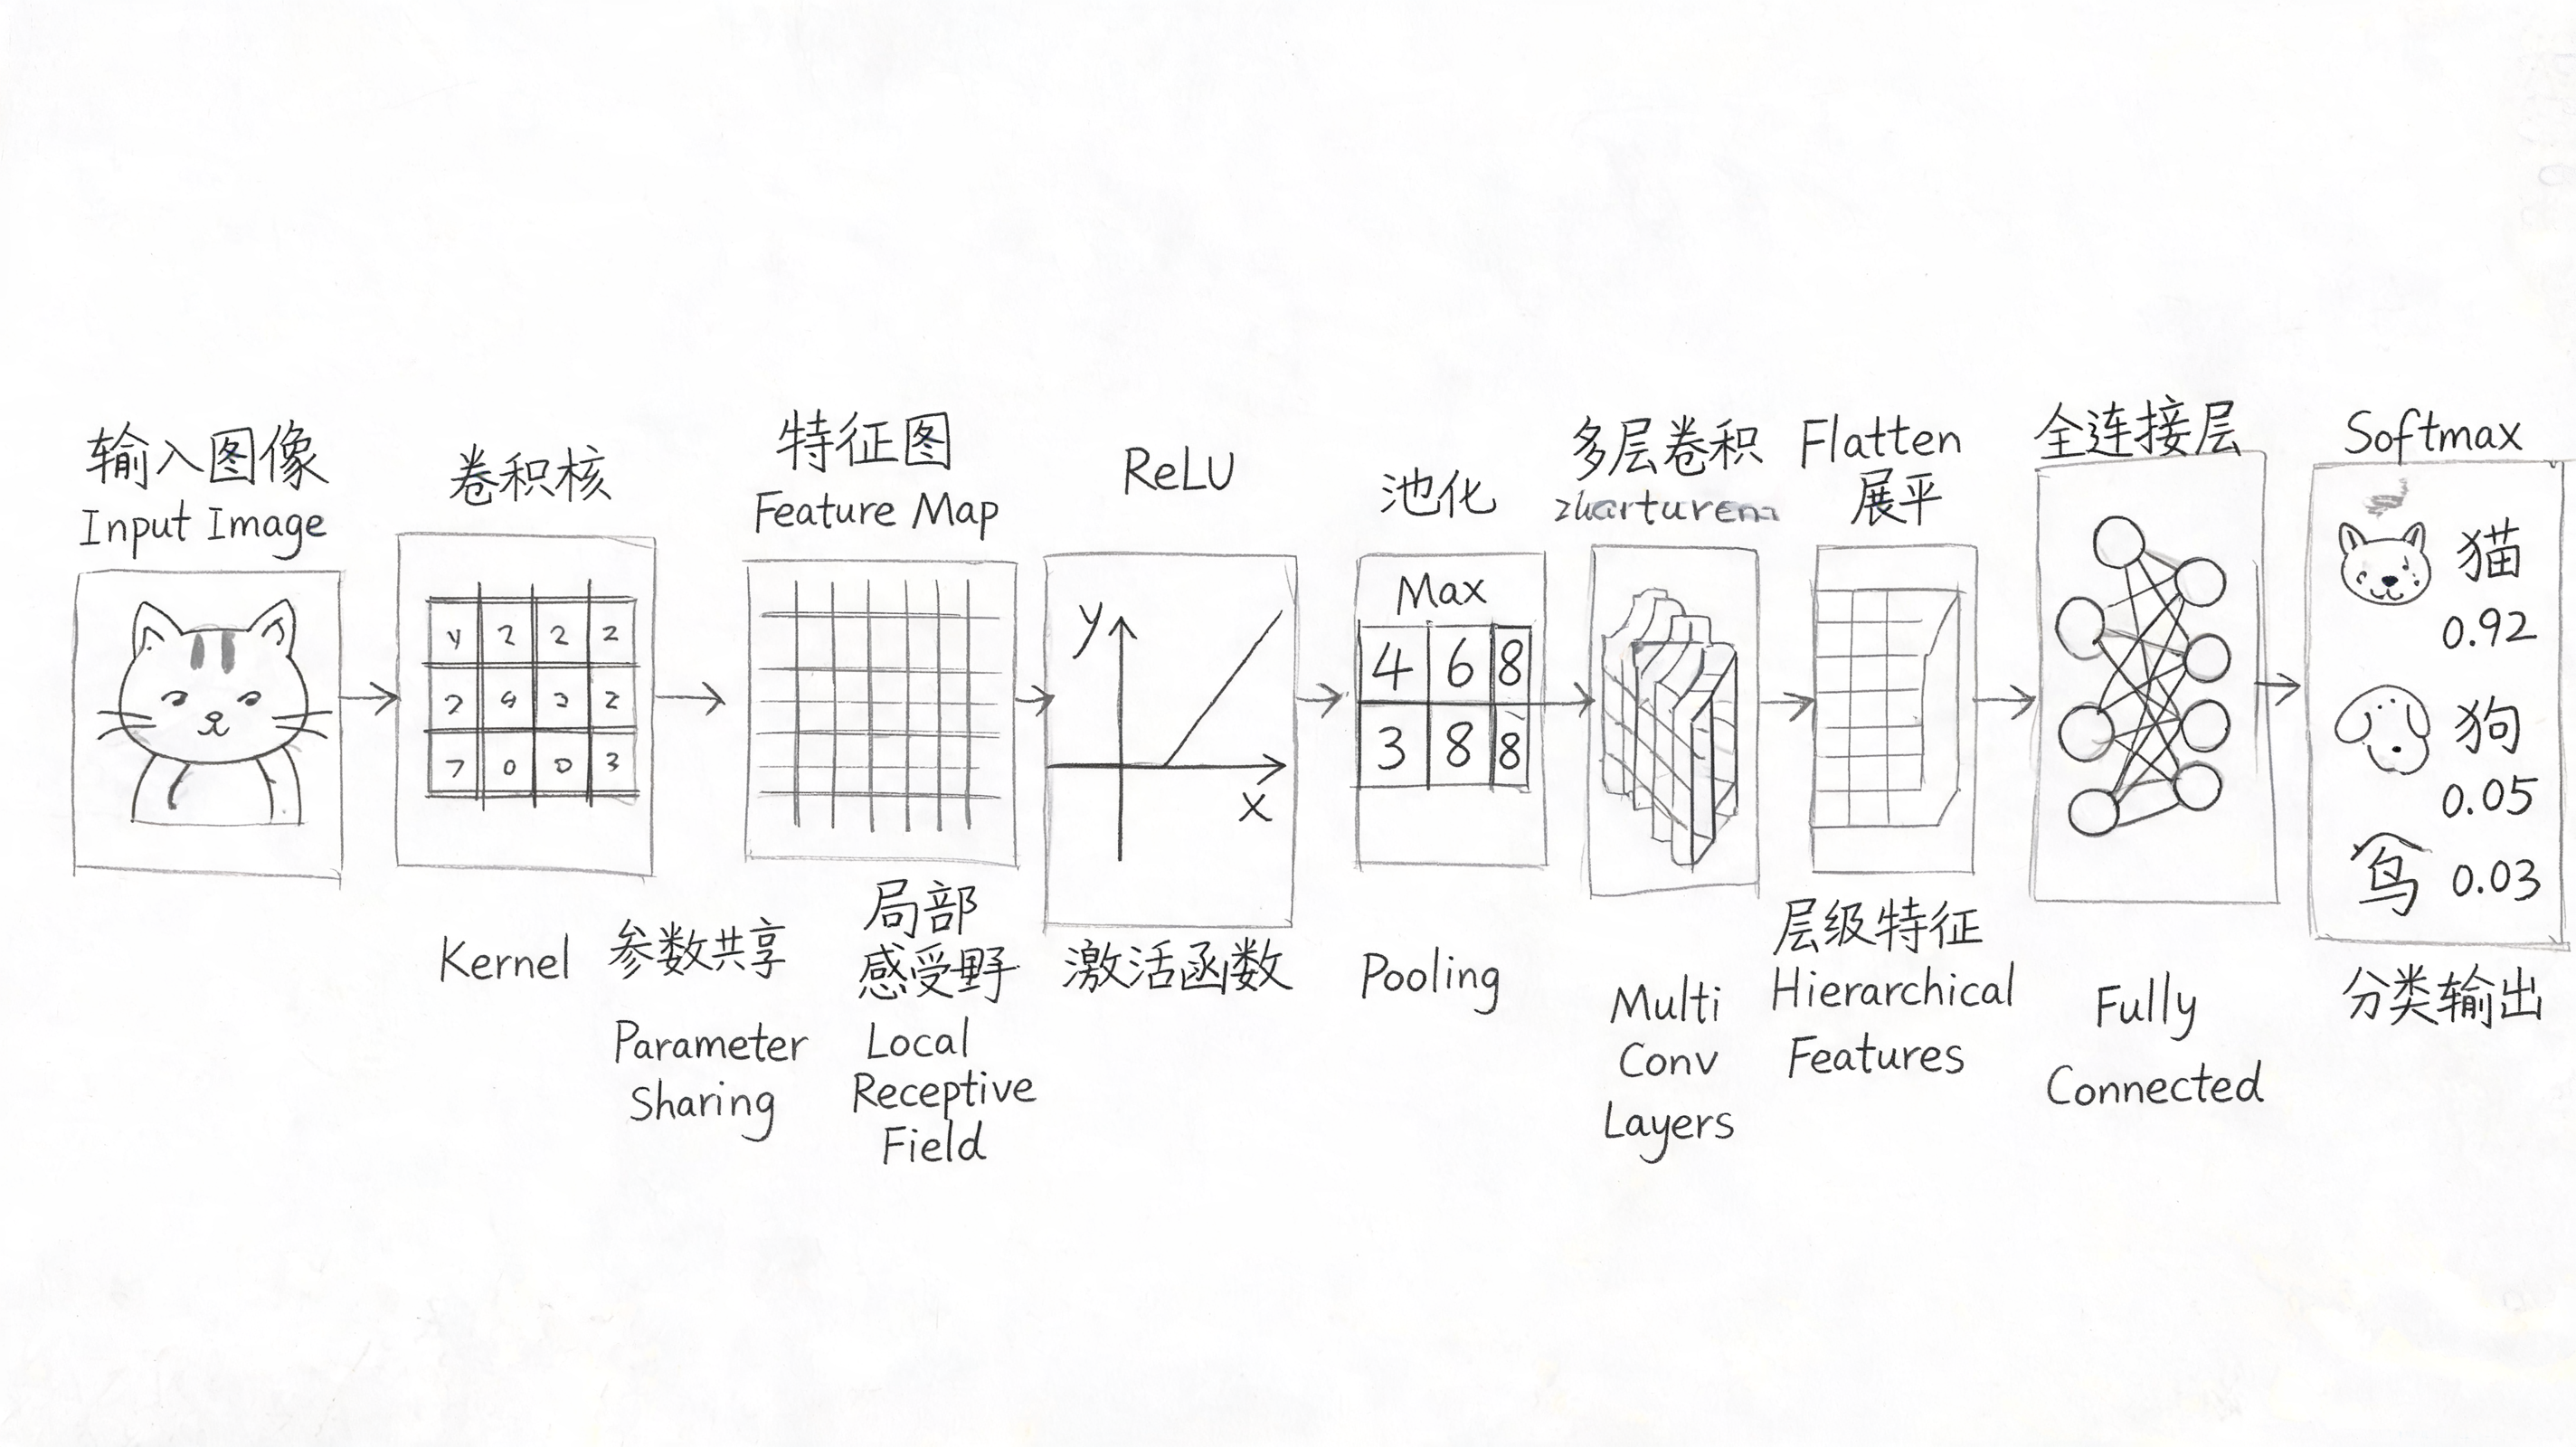
\includegraphics[width=\linewidth]{sample_cnn_sketch.png}
  \caption*{(a) 手绘草图输入}
\end{minipage}
\hfill
\begin{minipage}{0.32\textwidth}
  \centering
  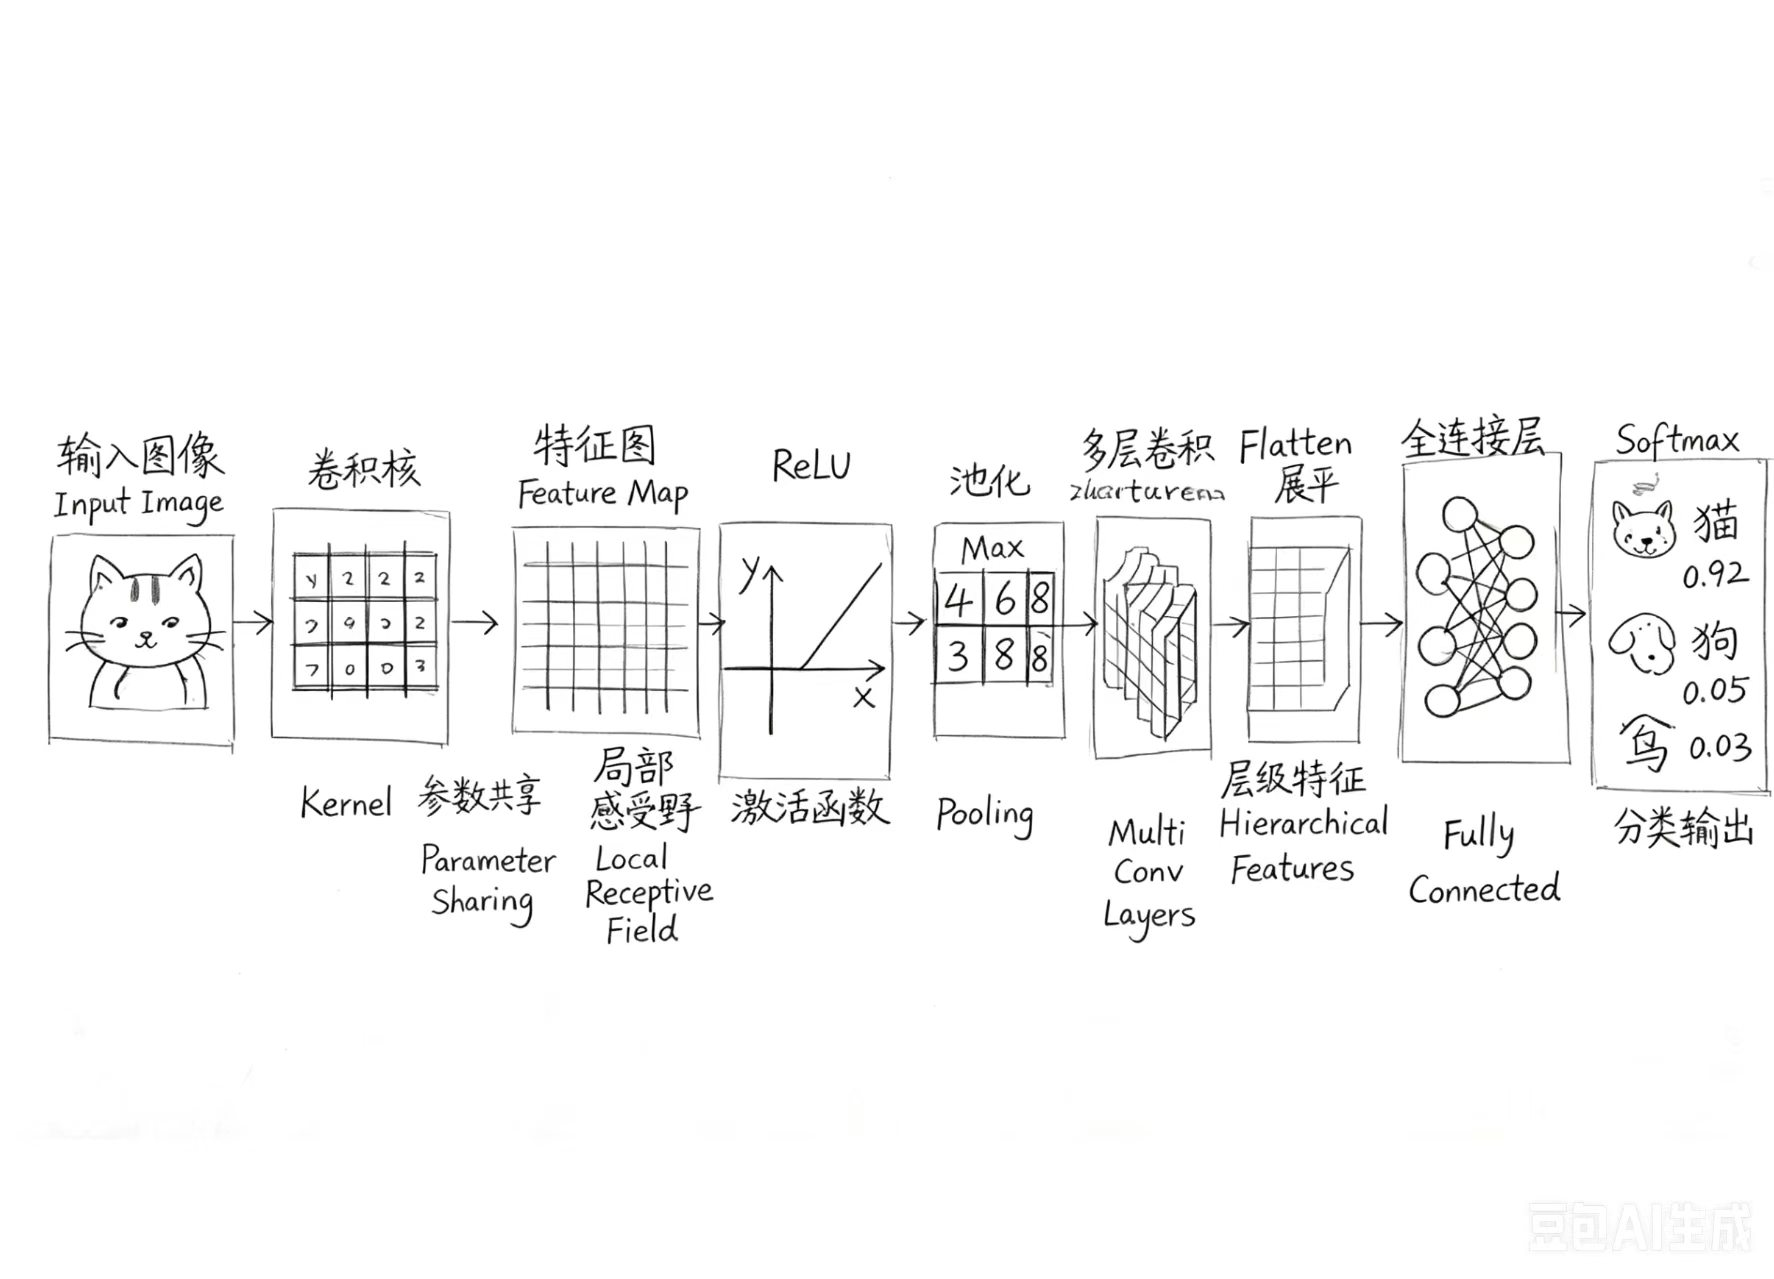
\includegraphics[width=\linewidth]{product_cnn_method.jpg}
  \caption*{(b) 结构化方法图}
\end{minipage}
\hfill
\begin{minipage}{0.32\textwidth}
  \centering
  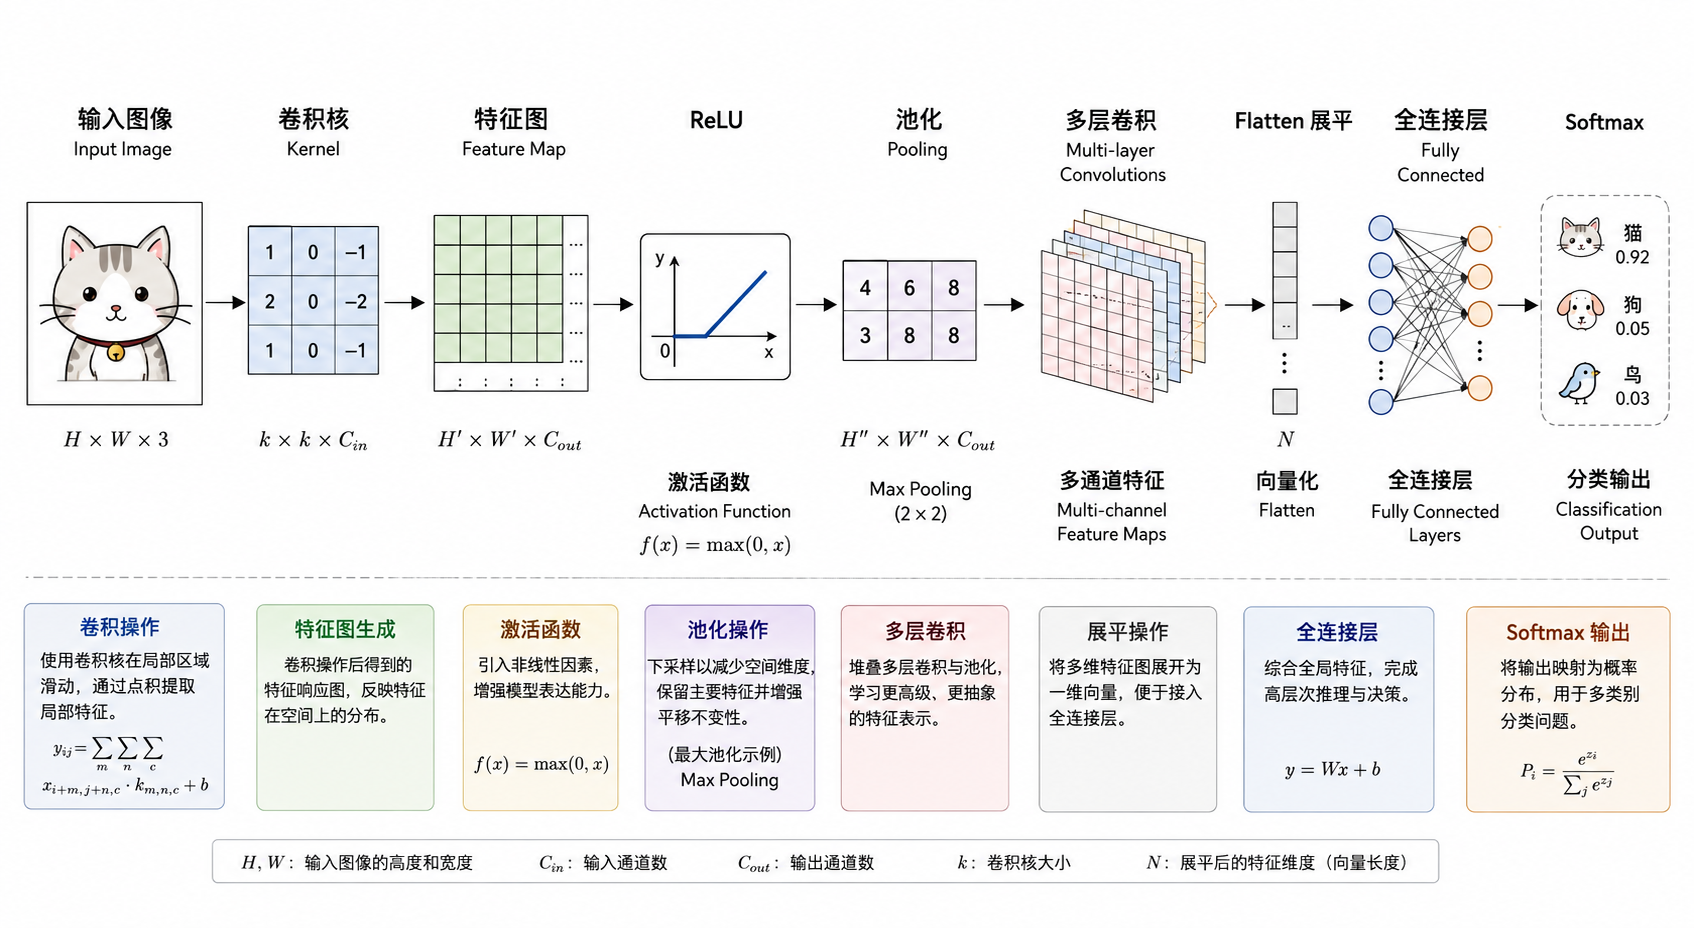
\includegraphics[width=\linewidth]{product_cnn_final.png}
  \caption*{(c) 终稿图效果}
\end{minipage}
\caption{交互式原型的输入与输出示例。}
\label{fig:product-demo}
\end{figure}

原型功能覆盖草图绘制、语音输入、文本修订、结构图生成、图形预览、结果导出和讲解生成。其应用价值在于，用户不需要先写完整需求文档，也不需要手工微调每个图形元素，而是可以通过自然讲述和粗略草图表达意图，再由系统生成可继续编辑的结构化结果。

\section{验收反馈补充}

验收阶段指出的核心问题是：研究内容需要更深入联系语音信息领域，而不是只把语音作为输入按钮。针对该反馈，报告正文补充了三方面内容。首先，选题背景从语音交互、人机自然交流和语音信号处理基础展开，说明语音技术是任务成立的重要基础。其次，方法部分将语音侧定义为语义锚点源，明确其在节点、关系、顺序和重点覆盖上的约束作用。最后，实验分析增加了语音单模态、早期融合和双源桥之间的差异解释，说明语音内容如何降低草图结构化的不确定性。

当前实验结果属于可控验证，对于真实语音识别和真实视觉解析的最终性能进行启发探索。后续会继续从真人语音、噪声条件、专业术语误识别、跨说话人差异和真实用户修改轨迹等方向进行完善拓展。

\section{小组成员分工}

\begin{table}[H]
\centering
\caption{小组成员分工}
\begin{tabular}{C{2.6cm}P{8.8cm}C{2.0cm}}
\toprule
成员 & 主要贡献 & 贡献度 \\
\midrule
gzp & 负责选题 idea、实验设计与执行、产品设计和报告主体组织。 & 1/3 \\
gcj & 负责汇报组织、实验方法沉淀与归纳，协助形成面向展示的技术表达。 & 1/3 \\
lky & 负责产品实现、报告完善和演示材料制作，支持系统闭环展示。 & 1/3 \\
\bottomrule
\end{tabular}
\end{table}

\bibliographystyle{plain}
\bibliography{references}

\end{document}
